%!TEX root = ../../Thesis.tex

\section{Experimental Evaluation}\label{sec:exp}

% %!TEX root = ../../Thesis.tex


Even though we describe the Serializability checking algorithm theoretically in subsection \ref{ssec:ser_checking} and showed the reductions for Prefix Consistency in subsection \label{ssec:pc} and Snapshot Isolation in subsection \label{ssec:si}, we should discuss about our actual implementations before discussing our experimental results.

After processing the history, we maintain $\so$, $\wro_{x}$ as relations in hashmaps for faster access. For relation set related operations, we implemented optimized algorithms for this hashmaps such as computing transitivity on the fly, checking inclusion, finding cycles. 

\subsection{Implementation for Serializability}\label{ssec:imp-ser}
We follow our algorithm \ref{seralgo:2} to implement this. The main difference to the pseudo-code is to reduce the storage complexity while doing the DFS search (demonstrated in figure \ref{ser_algo_example:3}), we maintain a state of the search in an optimized data structure. This data structure includes the sequence of choices till that point and the active variables $x$ which has a active $\wro_{x}$ between a \textsf{Write} inside of current serializable prefix and a \textsf{Read} outside of the prefix.

TODO: example

When we add a new transaction in the serializable prefix, we add it to the sequence of choices and update the active variable set.

When we backtrack, we read our history and remove the last choice of transaction and read the history and restore the previous active variable set.


\subsection{Implementation for Prefix Consistency}\label{ssec:imp-pc}

Even though we have a reduction for Prefix Consistency to Serializability, we implement a direct algorithm for it. We perform the reduction on the fly. We implement our serializable algorithm on a \emph{virtual} history where the a splited transaction $T$ is denoted by $(T, Read)$ and $(T, Write)$. 

\subsection{Implementation for Snapshot Isolation}\label{ssec:imp-si}

The algorithm for Snapshot Isolation is implemented similarly as Prefix Consistency. A splited transaction $T$ is denoted by $(T, Read)$ and $(T, Write)$. But two transactions those write on same variable, their split transactions can not interleave. So $\vartriangleright$ also checks if a $(T, Read)$ is includes, there is no $T'$ in the serializable prefix such that $T$ and $T'$ do not write on same variable.


\begin{figure}
\centering
 \begin{subfigure}{.33\textwidth}
  \resizebox{\textwidth}{!}{
   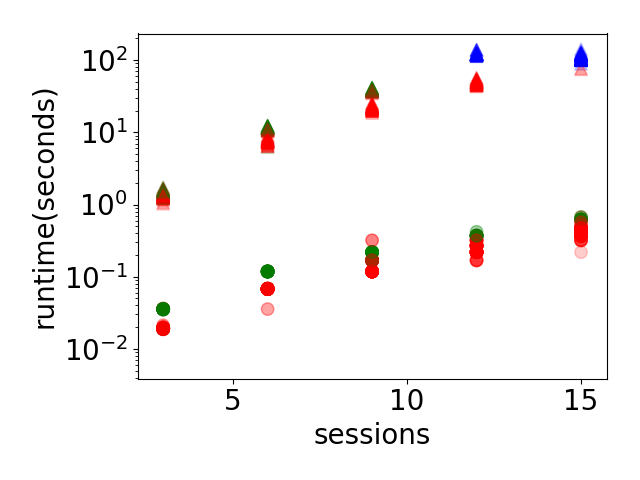
\includegraphics{Sources/transaction/plots/roachdb_sessions.png}
  }
  \caption{Sessions.}
  \label{ser_node_scale}
 \end{subfigure}
 \hspace{-3mm}
 \begin{subfigure}{.33\textwidth}
  \resizebox{\textwidth}{!}{
   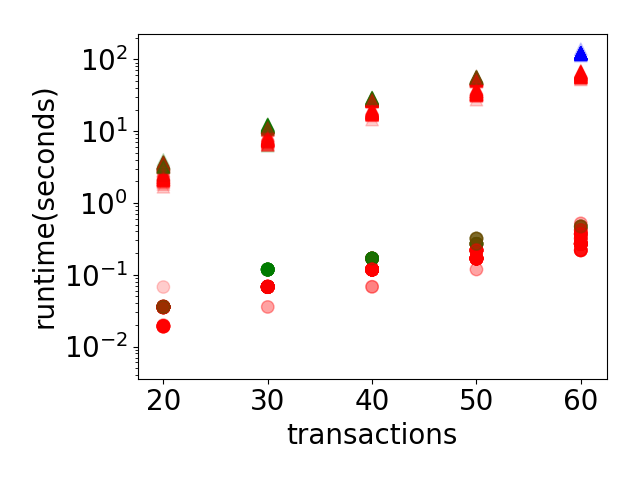
\includegraphics{Sources/transaction/plots/roachdb_transactions.png}
  }
  \caption{Transactions per session.}
  \label{ser_transaction_scale}
 \end{subfigure}

 \begin{subfigure}{.33\textwidth}
  \resizebox{\textwidth}{!}{
   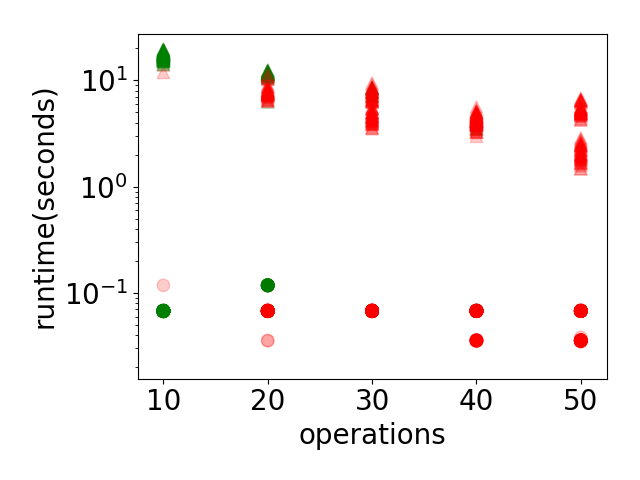
\includegraphics{Sources/transaction/plots/roachdb_operations.png}
  }
  \caption{Operations per transaction.}
  \label{ser_operation_scale}
 \end{subfigure}
 \hspace{-3mm}
 \begin{subfigure}{.33\textwidth}
  \resizebox{\textwidth}{!}{
   \includegraphics{Sources/transaction/plots/roachdb_variables.png}
  }
  \caption{Variables.}
  \label{ser_variable_scale}
 \end{subfigure}
% \begin{subfigure}{.33\textwidth}
%  \resizebox{\textwidth}{!}{
%   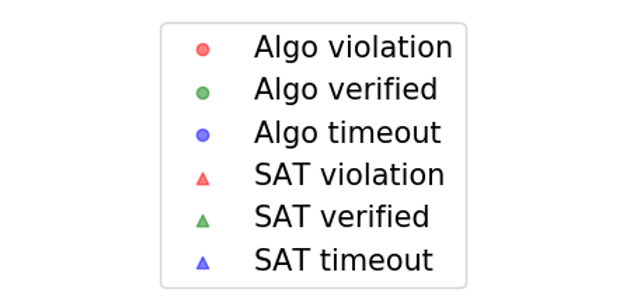
\includegraphics[scale=0.5]{plots/legends.png}
%  }
%  \caption{Legends}
%  \label{legend_1}
% \end{subfigure}
 \vspace{-3mm}
 \caption{Scalability of our algorithm for checking \textsc{Serializability} (Algorithm~\ref{seralgo:2}) with comparison to a SAT encoding. The x-axis represents the varying parameter while the y-axis represents the wall-clock time in logarithmic scale. The circular, resp., triangular, dots represent wall-clock times of our algorithm, resp., the SAT encoding. The red, green, and blue dots represent invalid, valid and resource-exhausted instances, respectively.}
 \label{ser_performace_scale}
 \vspace{-3mm}
\end{figure}


To demonstrate the practical value of the theory developed in the previous sections, we argue that our algorithms:
\begin{itemize}
 \item are efficient and scalable, %and they outperform a SAT encoding of the axioms in Section~\ref{sec:def},
 \item enable an effective testing framework allowing to expose consistency violations in production databases.
\end{itemize}

We focus on three of the criteria introduced in Section~\ref{sec:def}: \emph{serializability} which is NP-complete in general and polynomial time when the number of sessions is considered to be a constant, \emph{snapshot isolation} which can be reduced in linear time to serializability, and \emph{causal consistency} which is polynomial time in general.
%\footnote{Our implementation is publicly available. URL omitted to maintain anonymity.}. 
As benchmark, we consider histories extracted from three distributed databases: CockroachDB~\cite{cockroach}, Galera~\cite{galera}, and AntidoteDB~\cite{antidote}. %\footnote{The databases are deployed using Docker.}.
% snapshot isolation, and causal consistency, and histories extracted from three distributed databases, CockroachDB~\cite{cockroach}, Galera~\cite{galera}, and AntidoteDB~\cite{antidote}.
% which implement serializability~\cite{cockroach-claim}, snapshot isolation~\cite{galera-claim} and causal consistency~\cite{antidote-claim}, respectively (with the default configuration). Therefore, all experiments concerning SER, SI, or CC use histories of CockroachDB, Galera, and AntidoteDB, respectively.
%
% how the histories are generated and executed
%sessions are uniformly distributed among all nodes of the considered distributed database
Following the approach in Jepsen~\cite{jepsen},  histories are generated with random clients. For the experiments described hereafter, the randomization process is parametrized by: (1) the number of sessions ({\bf \#sess}), (2) the number of transactions per session ({\bf \#trs}), (3) the number of operations per transaction ({\bf \#ops}), and (4) an upper bound on the number of used variables ({\bf \#vars})\footnote{We ensure that every value is written at most once.}. For any valuation of these parameters, half of the histories generated with CockroachDB and Galera are restricted such that the sets of variables written by any two sessions are disjoint (the sets of read variables are not constrained). This restriction is used to increase the frequency of valid histories. 
%We also insert a random pause of at most 200 milliseconds between every two transactions within the same session.
%\begin{itemize}
% \item A session is generated by choosing uniformly at random the type of the operations in each transaction (read or write), the variable accessed by each operation, and a value for each write operation. We ensure that every value is written at most once by a client by maintaining a counter map for each variable. 
% \item Each session writes on specific non-overlapping sets of variables of equal size. Otherwise, everything is same as before. A read and write operation are chosen randomly.
%\end{itemize}
%We consider the second type of histories is to increase the number of valid histories in CockroachDB and Galera, because they often produce inconsistent histories. Each history are generated separately as first and then it is executed on the mentioned databases. We used Docker to deploy these distributed instances. 
%Also, we insert a random pause of at most 200 milliseconds between every two transactions within the same session so that the network does not clog up. 

%Then, each executed history is verified with 10 minutes of time limit, 10GB of memory limit and 10GB of file size limit(to avoid big CNF files).

% ser
In a first experiment, we investigated the efficiency of our serializability-checking algorithm (Algorithm~\ref{seralgo:2}) and we compared its performance with a direct SAT encoding\footnote{For each ordered pair of transactions $\tr_1$, $\tr_2$ we add two propositional variables representing $\tup{\tr_1,\tr_2} \in (\wro \cup \so)^+$ and $\tup{\tr_1,\tr_2} \in \CO$, respectively. Then we generate clauses corresponding to: (1) singleton clauses defining the relation $\wro \cup \so$ (extracted from the input history), (2) $\tup{\tr_1, \tr_2} \in \wro \cup \so$ implies $\tup{\tr_1, \tr_2} \in \CO$, (3) $\CO$ being a total order, and (4) the axioms corresponding to the considered consistency model. This is an optimization that does not encode $\wro$ and $\so$ separately, which is sound because of the shape of our axioms (and because these relations are fixed apriori).} of the serializability definition in Section~\ref{sec:def} (we used MiniSAT~\cite{DBLP:conf/sat/EenS03} to solve the SAT queries). We used histories extracted from CockroachDB which claims to implement serializability, acknowledging however the possibility of anomalies~\cite{cockroach-claim}. The sessions of a history are uniformly distributed among 3 nodes of a single cluster. To evaluate scalability, we fix a reference set of parameter values: {\bf \#sess}=6, {\bf \#trs}=30, {\bf \#ops}=20, and {\bf \#vars} = 60 $\times$ {\bf \#sess}, and vary only one parameter at a time. For instance, the number of sessions varies from 3 to 15 in increments of 3. 
We consider 100 histories for each combination of parameter values. The experimental data is reported in Figure~\ref{ser_performace_scale}. Our algorithm scales well even when increasing the number of sessions, which is not guaranteed by its worst-case complexity (in general, this is exponential in the number of sessions). Also, our algorithm is at least two orders of magnitude more efficient than the SAT encoding. While the performance of SAT solvers is known to be heavily affected by the specific encoding of the problem, we strove to make the SAT formula as succinct as possible and optimize its construction.
We have fixed a 10 minutes timeout, a limit of 10GB of memory, and a limit of 10GB on the files containing the formulas to be passed to the SAT solver. The blue dots represent resource-exhausted instances. The SAT encoding reaches the file limit for 148 out of 200 histories with at least 12 sessions (Figure~\ref{ser_node_scale}) and for 50 out of 100 histories with 60 transactions per session (Figure~\ref{ser_transaction_scale}), the other parameters being fixed as explained above. 
 % .(i.e.,  {\bf \#sess}=6, {\bf \#ops}=20, and {\bf \#vars} = 360).

We have found a large number of violations, whose frequency increases with the number of sessions, transactions per session, or operations per transaction, and decreases when allowing more variables. This is expected since increasing any of the former parameters increases the chance of interference between different transactions while increasing the latter has the opposite effect. The second and third column of Table~\ref{violation_stat} give a more precise account of the kind of violations we found by identifying for each criterion X, the number of histories that violate X but no other criterion weaker than X, e.g., there is only one violation to SI that satisfies PC.

%They show our algorithm outperforming SAT encoding by almost 100 times.   In the plots for session, transactions, and events, we see more red plots to the right, this is because increasing these parameters adds more concurrent collisions in the system. If the number of variables is increased, the collisions decrease. Therefore, in the plot of the number of variables, we see green plots in the right. 198 histories with very big SAT instances exhausted memory limit and the average total number of non-empty committed transactions in those histories is 360.

%The main drawback of the SAT encoding is to generate all boolean variables for all possible relation. Usually, just the generation part of the SAT verifier spends more time than our verifier algorithm. Since our algorithms for SER are polynomial time for a fixed number of sessions, their scalability when the number of sessions increases may be an issue, at least in theory. 
%To test our algorithm, we fixed a reference parameter of 6 sessions, 30 transactions per session, 20 operations per transactions, and 60 variables per session. For each parameter, we vary the number of sessions only, keeping the other parameters fixed with this reference parameter and execute 100 different histories (50 of the first type of history and 50 of the second type) for each of them. To complete, we did similar experiments for other parameters as well. Our experimental data are plotted in Figure~\ref{ser_node_scale},~\ref{ser_transaction_scale},~\ref{ser_operation_scale}, and~\ref{ser_variable_scale}. The circular dots are our algorithm runtime, the triangle dots are SAT runtime. We plotted the varying parameter on the x-axis and plotted the verification duration on the y-axis in logarithmic scale. They show our algorithm outperforming SAT encoding by almost 100 times.  The red, green and blue plots are invalid, valid and resource exhausted instances. In the plots for session, transactions, and events, we see more red plots to the right, this is because increasing these parameters adds more concurrent collisions in the system. If the number of variables is increased, the collisions decrease. Therefore, in the plot of the number of variables, we see green plots in the right. 198 histories with very big SAT instances exhausted memory limit and the average total number of non-empty committed transactions in those histories is 360.


\begin{figure}
 \begin{subfigure}{.33\textwidth}
  \resizebox{\textwidth}{!}{
  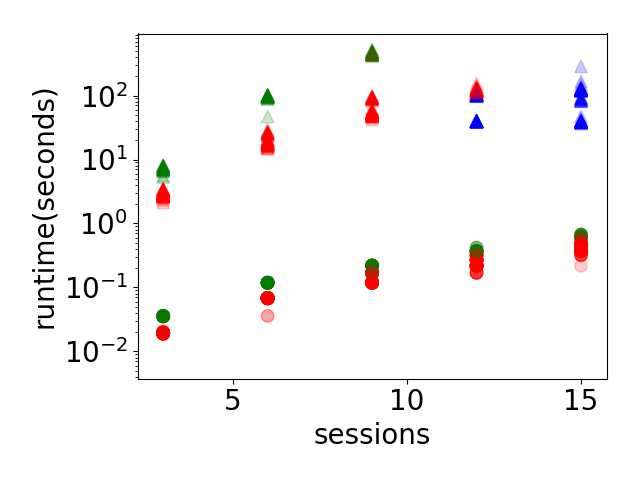
\includegraphics{Sources/transaction/plots/roachdb_si_sessions.png}
  }
  \caption{Checking SI (CockroachDB)}
  \label{roach_si_node_scale}
 \end{subfigure}
 \hspace{-2mm}
 \begin{subfigure}{.33\textwidth}
  \resizebox{\textwidth}{!}{
   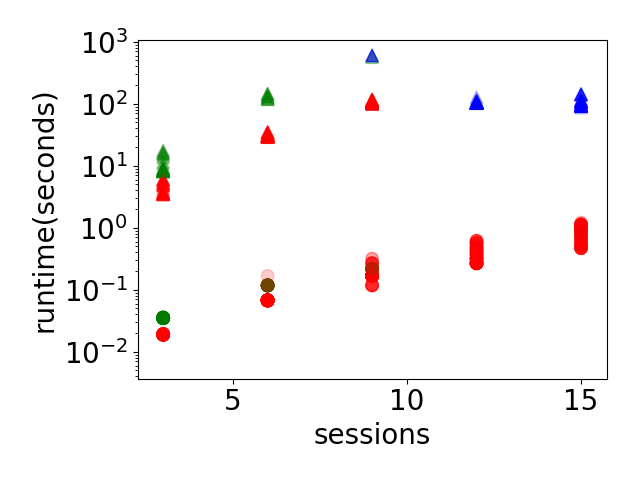
\includegraphics{Sources/transaction/plots/galera_sessions.png}
  }
  \caption{Checking SI (Galera)}
  \label{galera_si_node_scale}
 \end{subfigure}
  \hspace{-2mm}
 \begin{subfigure}{.33\textwidth}
  \resizebox{\textwidth}{!}{
   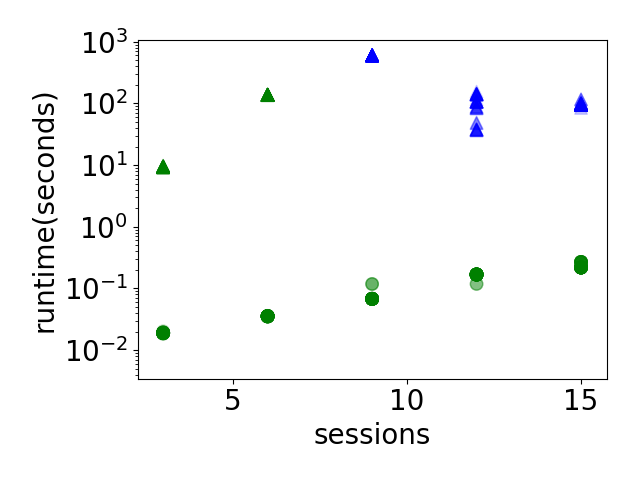
\includegraphics{Sources/transaction/plots/antidote_sessions.png}
  }
  \caption{Checking CC (AntidoteDB)}
  \label{cc_session_scale}
 \end{subfigure}
% \vspace{-3mm}
% \begin{subfigure}{.33\textwidth}
%  \resizebox{\textwidth}{!}{
%   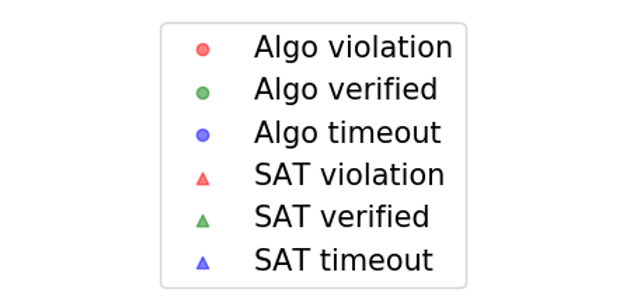
\includegraphics[scale=0.5]{plots/legends.png}
%  }
%  \caption{Legends}
%  \label{legend_2}
% \end{subfigure}
% \vspace{-2mm}
 \caption{Scalability of our algorithms for checking \textsc{Snapshot isolation} (Section~\ref{ssec:si}) and  \textsc{Causal consistency} (Algorithm~\ref{ccalgo:1}) with comparison to a SAT encoding. The x-axis represents the varying parameter while the y-axis represents the wall-clock time in logarithmic scale. The circular, resp., triangular, dots represent wall-clock times of our algorithm, resp., the SAT encoding. The red, green, and blue dots represent invalid, valid and resource-exhausted instances, respectively.}
 \label{si_cc_performace_scale}
\end{figure}

The second experiment measures the scalability of the SI checking algorithm obtained by applying the reduction to SER described in Section~\ref{ssec:si} followed by the SER checking algorithm in Algorithm~\ref{seralgo:2}, and its performance compared to a SAT encoding of SI. Actually, the reduction to SER is performed on-the-fly, while traversing the history and checking for serializability (of the transformed history). The SAT encoding follows the same principles as in the case of serializability. We focus on its behavior when increasing the number of sessions (varying the other parameters leads to similar results). As benchmark, we used the same CockroachDB histories as in Figure~\ref{ser_node_scale} and a number of histories extracted from Galera\footnote{In order to increase the frequency of valid histories, all sessions are executed on a single node.} whose documentation contains contradicting claims about whether it implements snapshot isolation~\cite{galera-claim,galera-notclaim}. We use 100 histories per combination of parameter values as in the previous experiment. The results are reported in Figure~\ref{roach_si_node_scale} and Figure~\ref{galera_si_node_scale}. We observe the same behavior as in the case of SER. In particular, the SAT encoding reaches the file limit for 150 out of 200 histories with at least 12 sessions in the case of the CockroachDB histories, and for 162 out of 300 histories with at least 9 sessions in the case of the Galera histories. The last two columns in Table~\ref{violation_stat} classify the set of violations depending on the weakest criterion that they violate.

We also evaluated the performance of the CC checking algorithm in Section~\ref{sec:general} when increasing the number of sessions, on histories extracted from AntidoteDB, which claims to implement causal consistency~\cite{antidote-claim}. The results are reported in Figure~\ref{cc_session_scale}. In this case, the SAT encoding reaches the file limit for 150 out of 300 histories with at least 9 sessions. All the histories considered in this experiment are valid. However, when experimenting with other parameter values, we have found several violations. The smallest parameter values for which we found violations were 3 sessions, 14 transactions per session, 14 operations per transaction, and 5 variables. The violations we found are also violations of Read Atomic. For instance, one of the violations contains two transactions $\tr_1$ and $\tr_2$, each of them writing to two variables $x_1$ and $x_2$, and another transaction $\tr_3$ that reads $x_1$ from $\tr_1$ and $x_2$ from $\tr_2$ ($\tr_1$ and $\tr_2$ are from different sessions while $\tr_3$ is an $\so$ successor of $\tr_1$ in the same session). These violations are novel and they were confirmed by the developers of AntidoteDB.

%are of this form - two committed transactions, $\tr_1$ and $\tr_2$, write on two variables $x_1$ and $x_2$, then one another transaction, $\tr_3$, reads $x_1$ from $\tr_1$ and $x_2$ from $\tr_2$. These violations are of ReadAtomic consistency. These violations are novel and they were confirmed by the developers of AntidoteDB.
%Similar to SER, we experimented for SI algorithm on Galera and CC algorithm on AntidoteDB as well. 
%%We chose 1 node for Galera (to get more valid histories) and 3 nodes for AntidoteDB. Since SI algorithm is similar to SER and CC algorithm is polytime, we only experimented on the scaling the number of sessions keeping the other parameters fixed. Figure~\ref{si_cc_performace_scale} shows they are performed as expected under session scaling and outperformed SAT encoding. Similar to SER, we also saw some memory limit exhausting SAT instances. 
%162 out of 250 and 150 out of 250 histoies exhausted resource limit for the SI verification of Galera and the CC verification of AntidoteDB respectively. The average total number of transactions in such histories are 402 and 361 for Galera and AntidoteDB respectively.

%Our testing infrastructure was able to find violations of all these criteria meaning that none of the databases we considered satisfies the guarantees stated in the documentation. In Table~\ref{violation_stat}, the violations are very frequent and much weaker than the guarantees for CockroachDB and Galera (more than half of the generated histories) and very rare for AntidoteDB. Actually, for AntidoteDB, the smallest parameter values for which we found violations were 3 sessions, 14 transactions per session, 14 operations per transaction, and at most 5 variables and these violations are of ReadAtomic consistency. These violations were exposed with a frequency of around 20 out of 1000 histories. In the case of CockroachDB, the documentation admits possible anomalies while in the case of Galera, consistency violations were already reported in an open issue on Github~\cite{galera-issue}. The CC violations we found in AntidoteDB are novel and have been confirmed by its developers.

%\begin{figure}
% \resizebox{.45\textwidth}{!}{
%  \includegraphics{plots/roachdb_variables}
% }
% \vspace{-3mm}
% \caption{TODO: add figure Bicomponent decomposition comparison}
% \label{bic_plot}
% \vspace{-2mm}
%\end{figure}

%TODO We don't consider the communication graph story since this requires a deployment on a large cluster which our proof of concept prototype cannot handle.

The refinement of the algorithms above based on communication graphs, described in Section~\ref{sec:communication}, did not have a significant impact on their performance. The histories we generated contained few biconnected components (many histories contained just a single biconnected component) which we believe is due to our proof of concept deployment of these databases on a single machine that did not allow to experiment with very large number of sessions and variables. 

%Lastly, we used our bicomponent technique to scale our algorithm for large histories with relatively less shared variables across the sessions. We present the plot for the runtime of the algorithm with and without bicomponent decomposition in Figure~\ref{bic_plot}.

\begin{table}
\caption{Violation statistics. The ``disjoint writes'' columns refer to histories where the set of variables written by any two sessions are disjoint.}
\small{
 \begin{tabular}{|l|c|c|c|c|c|}
  \hline
  & \multicolumn{2}{c|}{Serializability checking} & \multicolumn{2}{c|}{Snapshot Isolation checking} \\
  \hline
  Weakest                  & CockroachDB     & CockroachDB     & Galera      & Galera                \\
  criterion violated         & (disjoint writes) & (no constraints) & (disjoint writes) & (no constraints)  \\
  \hline
  Read Committed     &             &             & 19          & 50              \\
  Read Atomic        & 180         & 547         & 91          & 139                \\
  Causal Consistency            & 339         & 382         & 88          & 43                  \\
  Prefix Consistency            & 2           & 7           &             &                    \\
  Snapshot Isolation &             & 1           &             & 1                   \\
  Serializability      & 25          &             &            &                     \\
  \hline
%  Serializable      & 454         & 63          & 48          & 16                \\
  \hline
  Total number of violations           & 546/1000        & 937/1000        & 198/250         & 233/250              \\
  \hline
 \end{tabular}
 }
% \vspace{1mm}
 \label{violation_stat}
\end{table}

%We also computed the overheads of running our algorithms on real executions. On the CockroachDB (serializability) it is 0.83\% in average \ie out algorithm takes in average 0.83\% of the execution duration of one single history. For Galera, this value 4.6\%. For AntidoteDB, it is 2.5\%.  


%We verified three databases - AntidoteDB for Causal consistency, Galera for Snapshot isolation, CockroachDB for Serializability. We used Docker to deploy distributed instances. Using our implementation we found,
%
%\begin{itemize}
% \item Rarely AntidoteDB fails to maintain Casusal consistency for big parameters for transactions per node and operations per transaction. In our testing, the lowest paramter that violate this is (X, X, X, X). We tested XXX many case of that paramter and found YYY many violation. We also observed, the violation actually is of Read Atomic. 
% \item We tested 17809 many histories for Galera. 8991 many of them read writes from aborted transactions, read from other transactions after a write internally or do not maintain repeatable read. As of the Snapshot isolation we found 2301 many violations among 8818 many case which do not violate the above case.
% \item We tested many histories of CockroachDB. It never violate the cases mentioned for Galera. But out of 17000 many executions we found 12084 violations of Serializability.
%\end{itemize}
%
%
%
%
%
%We choose $(3,5,5,5)$ as our base parameters for number of nodes, number of transactions per node, number of operations per transaction, number of variables resp. We scale only one parameters and fix other parameter. For each database, we generated 1000 histories for each paramter and executed the generated histories and record the observed histories.
%
%Then we used our implementation to verify the said executions and recorded the durations for each history our algorithm took to finish. We plot the mean duration of each paramter in figure \ref{performace_scale}.
%
%
%
%We also compared our implementation with SAT version of the problem. We encode the problem in SAT and solved it with MiniSAT. We randomly picked from 500 from each set of verified and violated executions and solved with MiniSAT. We compare the runtime of SAT with our implementation in figure \ref{vs_sat}. 
